\chapter{Verification of confirmations}

\section{Network Model}

We assume a multihop network with a set $ S = \{s1,...,s_{n}\} $ of $n$
sensor nodes. The network is organized in a tree topology, with the
base station as the root of the tree. The trusted querier resides
outside of the network \& has more computation, storage capacity 
then the sensor nodes in the network. The base station and the 
querier knows total number of sensor nodes $n$ and the network 
topology. All the wireless comuunication is peer-to-peer and we do 
not consider local wireless broadcast. We also assume that the
querier has the capacity to do peer to peer communication with 
every sensor node in the network.

\subsection{Sensor Nodes}

	We assume that each sensor node has a unique identifier $s$ and
	shares a unique secret symmetric key $K_{s}$ with the querier. 
	We assume all the sensor nodes are capable of doing symmetric-
	key encryption and symmetric key decryption. They are also
	capable of computing collision-resistant cryptographic hash 
	function $H$. We also assume that if the sensor node has to send 
	multiple messages to its parent it can combine those messages 
	into single packet.

\subsection{Commitment trees} % (fold)
\label{sub:Commitment trees}
		
	The aggregation tree is a physical network over which all the
	communication happens while the commitment tree is a logical
	network on top of aggregation tree. In the similar manner, 
	vertices in a commitment tree is a logical element in a graph 
	while a sensor node is a physical device. 

	The commitment trees have the following properties. 
	At most there will be $\lceil lg  n \rceil$ commitment trees in the forest for an aggregation tree with $n$ sensor nodes.
	The binary representation of the number of sensor nodes $n$ in the network indicates the number of commitment trees in the forest. It also indicates the height of all the commitment trees in the forest. 
	For instance, if there are $ 11_{10} = 1011_{2} $ sensor nodes in the aggregation tree then there will be three commitment trees in the forest. From those three commitment trees, one will be of height three, one will be of height one and one will be of height zero.
	At most there will be $n + ( n - 1 )$ vertices in the forest of commitment trees for an aggregation tree with $n$ sensor 
	nodes.

	\textit{It is also possible that only one sensor node $s$ in the aggregation tree, will be the root vertex of all the commitment trees in the forest.} 

	\textit{It is also poosible that all the internal vetices in the commitment tree are of different sensor nodes in the aggregation tree.}

% subsection Commitment trees (end)

\subsection{Collections of confirmations}
After each sensor node $s$ has successfully performed the 
verification step for its leaf vertex $u_{s}$, it sends an 
authentication code to its parent in the aggregation tree.
The authentication code for sensor node $s$ is MAC$_{K_{s}}(N||ACK)$
where ACK is an acknowledgemnet message, N is the query nounce and $K_{s}$ 
is the secret key that sensor node $s$ shares with the trusted querier. Once
an internal sensor node $s$ in the aggregation tree has received the
authentication codes from all of its descendants, it computes the XOR of its 
own authentication code with all the received authentication codes, and 
forwards the result to its parent. Finally, the querier will receive a 
single authentication code from the base station that consists of the XOR of 
all the authentication codes received in the network. 

\subsection{Verification of confirmations}
Since the querier knows the secret key $K_{s}$ for each sensor node $s$ and 
it also knows the topology of the commitment trees in the forest, it can
simulate the commitment trees in the forest. The querier simulates the 
commitment trees in the forest by computing the following authentication 
codes\\
MAC$_{K_{1}}(N||ACK)\,\oplus\,$ 
MAC$_{K2}(N||ACK)\,\oplus\,$
...
$\,\oplus\,$
MAC$_{K_{n}}(N||ACK)$ ; \\
MAC$_{K_{1}}(N||NACK)\,\oplus\,$ 
MAC$_{K2}(N||NACK)\,\oplus\,$
...
$\,\oplus\,$
MAC$_{K_{n}}(N||NACK)$  \\
and creates two simulated commitment trees, one with the authentication codes of ACK messages and one with the authentication codes of NACK messages; where ACK is an acknowledgemnet message, NACK is a negative acknowledgemnet message \& N is the query nounce. Then the querier merges all the commitment trees in the forest simulated with ACK messages, by taking XOR of the root of all the commitment trees in the forest and calculates a single root authentication code for the forest simulated with ACK messages. The querier does the same procedure for the simulated commitment trees' forest with NACK messages. The querier stores all the simulated commitment trees and root authentication codes in the memory. 

The querier receives a signle root authentication code from the base station in the collection of confirmation messages step. The querier compares the received root authentication code with its simulated root authentication code of ACK message commitment trees' forest. If those two values match it means every node in the network sent ACK message during collection of confirmation step. If those two values do not match it means one or more nodes in the network sent NACK message during collection of confirmation step. In the case where root authentication codes do not match, the querier will proceed futher to find out which node or nodes in the network sent NACK message.

To find out which node or nodes in the network reported NACK message, the querier will ask the base station to send the authentication codes of all the commitment trees' root in the forest. After receiving the authentication codes from the base station, the querier will compare those authentication codes with its simulated authentication codes of ACK trees. After this comparision, whose authentication codes do not match, the querier will classify those trees as BAD TREES in the commitment forest. 

Then the querier will compare the authentication codes of those BAD TREES with its simulated authentication codes for NACK trees. If any of those authentication codes match it means all the nodes in that commitment tree sent NACK message during collection of confirmation stpe. If those values do not match then the querier will proceed furhter to find the senosr node or nodes who reported NACK message in BAD TREES.

To find the sensor node or nodes who sent NACK messages in the BAD TREES, the querier will ask the root nodes of the BAD TREES to send the authentication codes of their childern. The querier will compare those authentication codes with relevant simulated commitment trees in the forest. First the querier will compare those authentication codes with simulated trees with NACK messages. If any of those childern's authentication codes match with the authentication codes from simulated trees of NACK messages, it means all the nodes rooted in that subtree sent NACK message. If those authentication codes do not match then the querier will compare those authentication codes with simulated trees of ACK messages. The querier will look for the node or nodes whose authentication codes do not match and then the querier will add those subtree rooted at those nodes as BAD TREE. Then the querier will repeat this process recursively untill it finds the node or nodes who reported NACK messages.

\subsection{Analysis} % (fold)
\label{sub:analysis}

To simulate the commitment trees in the forest the querier has to do the following calculations. Suppose there are $n$ sensor nodes in the network, means there will be at most $\lceil lg n \rceil$ commitment trees in the forest. If there are $n^{'}$ leaves in each commitment tree in the forest then the height($h^{'}$) of each commitment tree will be $lg(n^{'})$ and the number of intermediate vertices ($i^{'}$) in the network will be ($ 2^{h^{'}} - 1 $). So, there will be total of  $ (n^{'} + i^{'}) $ * $\lceil lg  n \rceil $  vertices in the forest. As the querier needs to simulate two commitment trees one for ACK messages and one for NACK messages it has to do ( $ 2 * (n^{'} + i^{'}) * \lceil lg  n \rceil $ ) calculations.

As we know from the properties of commitment trees, at most there 
will be $n + ( n - 1 )$ vertices in the forest of commitment trees 
for an aggregation tree with $n$ sensor nodes. So, the querier has
to do $ 2 * ( n + ( n - 1 ) )$ calculations and it also need that much memory space to store those values.
% subsection analysis (end)

\begin{figure}[t]
	\centering
		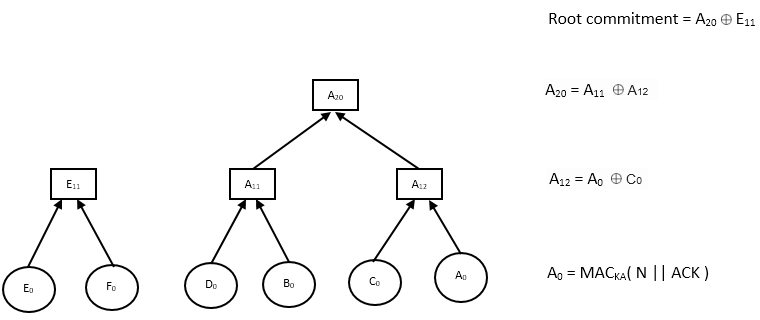
\includegraphics[width=0.8\textwidth]{ack.png}\\
		\caption{Simulated commitment tree with ACK messages}
	\label{fig:figure1}
\end{figure}

\begin{figure}[t]
	\centering
		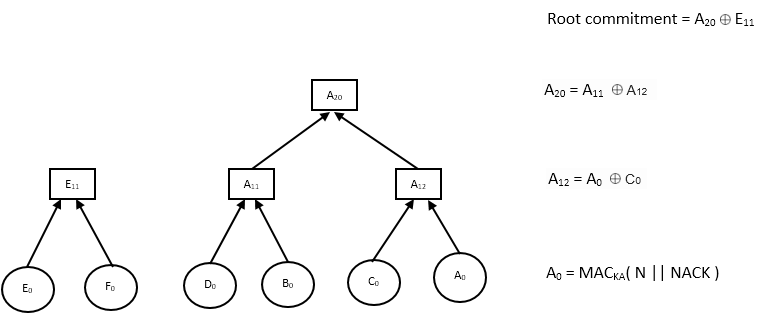
\includegraphics[width=0.8\textwidth]{nack.png}\\
		\caption[Simulated commitment tree with NACK messages]{Simulated commitment tree with NACK messages}
	\label{fig:figure1}
\end{figure}

